% !TEX root = thesis.tex

\chapter{Search System for Law Enforcement}
\label{ch:7}

% details from the aipr papers about the law enforcement portal, plus new info + screenshots
\begin{figure}[Ht!]
  \begin{center}
    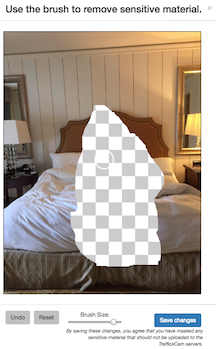
\includegraphics[width=.7\columnwidth]{figures/chapter6/masking.png}
 \end{center}
  \caption{Members of law enforcement mask off any sensitive content from their query images prior to the image being submitted to the server.}
  \label{fig:masking}
\end{figure}

Members of law enforcement who have been verified as working on sex trafficking cases can be granted access to the TraffickCam law enforcement portal. The law enforcement portal allows investigators to either browse all of the hotel room images that fit a text or geographic query, or to browse the images that are most similar to a query image. When an investigator provides a query image, they first mask off any sensitive regions of the image, as in Figure~\ref{fig:masking}. This masking occurs before the image content ever leaves the investigator's computer; therefore, sensitive data is never transmitted or stored by the TraffickCam system. The masked image is then submitted to the TraffickCam server, where image features are extracted and compared to the database of TraffickCam images in order to provide the investigator with a list of similar images and hotels.

The TraffickCam search interface allows law enforcement to retrieve these search results for a masked query image at a national scale in a matter of seconds. This search is based on features learned from a neural network trained on the TraffickCam dataset, as described in Section~\ref{methodology}, and the search index is implemented using the Faiss library for efficient search~\cite{faiss}.